
Ажилтны Гүйцэтгэлийн Үнэлгээний Систем нь бизнесийн байгууллагуудын ажилтнуудын гүйцэтгэлийг үнэлэх, хянах, удирдах үйл явцыг хялбаршуулах зорилготой вэб-д суурилсан програм юм. Энэхүү систем нь \textbf{үйлчлүүлэгч-серверын архитектур}-ыг дагаж, \textbf{микро үйлчилгээнд тулгуурласан арын хэсэг} болон \textbf{орчин үеийн урд тал}-тай бөгөөд хөгжүүлэлт, туршилт, үйлдвэрлэлийн орчинд тогтвортой байдлыг хангахын тулд контейнержуулалтыг ашигладаг. Доор архитектур, бүрэлдэхүүн хэсгүүд болон тэдгээрийн харилцан үйлчлэлийн тоймыг харуулав.

\subsection*{1. Системийн Тойм}
\begin{itemize}
    \item \textbf{Зорилго}: Хүний нөөцийн менежерүүд болон багийн ахлагчдад урьдчилан тодорхойлсон хэмжүүрүүд (жишээ нь, зорилго, KPI, санал хүсэлт) дээр үндэслэн ажилтны гүйцэтгэлийг үнэлэх, тайлан гаргах, ажилтнуудад өөрийгөө үнэлэх хэрэгсэл өгөх боломжийг олгох.
    \item \textbf{Гол Онцлогууд}:
    \begin{itemize}
        \item Хэрэглэгчийн баталгаажуулалт ба дүрд суурилсан хандалтын хяналт (жишээ нь, Админ, Менежер, Ажилтан).
        \item Гүйцэтгэлийн хэмжүүр, үнэлгээ, санал хүсэлтийн CRUD үйлдэл.
        \item Гүйцэтгэлийн чиг хандлага, тайланг харуулах хяналтын самбар.
        \item Үнэлгээний хугацаа, шинэчлэлтүүдийн мэдэгдэл.
    \end{itemize}
    \item \textbf{Байршуулалт}: Docker ашиглан контейнержуулсан бөгөөд хөгжүүлэлт, туршилт, үйлдвэрлэлийн орчинд тогтвортой, өргөтгөх боломжтой.
\end{itemize}

\subsection*{2. Архитектурын Бүрэлдэхүүн Хэсгүүд}

\subsubsection*{2.1 Урд Тал (Үйлчлүүлэгчийн Давхарга)}
\begin{itemize}
    \item \textbf{Технологи}: Next.js ба Tailwind CSS
    \item \textbf{Тодорхойлолт}: Урд тал нь Next.js (React-д суурилсан framework) ашиглан бүтээгдсэн нэг хуудасны програм (SPA) бөгөөд Tailwind CSS-ийн тусламжтайгаар хариу үйлдэл сайтай, орчин үеийн UI-тай.
    \item \textbf{Үүрэг}:
    \begin{itemize}
        \item Гүйцэтгэлийн үнэлгээний хяналтын самбар, маягт, тайланг харуулах.
        \item Хэрэглэгчийн харилцан үйлдлийг удирдах (жишээ нь, үнэлгээ илгээх, санал харах).
        \item RESTful API-аар дамжуулан back endтай харилцах.
    \end{itemize}
    \item \textbf{Гол Онцлогууд}:
    \begin{itemize}
        \item Сервер талын рендеринг (SSR) болон статик сайтын үүсгэлт (SSG) нь гүйцэтгэлийг оновчтой болгодог.
        \item Tailwind CSS нь төхөөрөмжүүдийн хооронд тогтвортой, өөрчлөх боломжтой загварыг хангана.
    \end{itemize}
\end{itemize}

\subsubsection*{2.2 back end (Серверын Давхарга)}
\begin{itemize}
    \item \textbf{Технологи}: Go (Golang) ба Gin, GORM, JWT
    \item \textbf{Тодорхойлолт}: back end нь Go-д бичигдсэн өндөр гүйцэтгэлтэй RESTful API сервер бөгөөд Gin-ийг чиглүүлэлт болон middleware-д, GORM-ийг өгөгдлийн сангийн харилцан үйлдэлд, JWT-ийг аюулгүй баталгаажуулалтад ашигладаг.
    \item \textbf{Үүрэг}:
    \begin{itemize}
        \item Гүйцэтгэлийн үнэлгээний бизнесийн логикийг удирдах (жишээ нь, оноо тооцоолох, санал хадгалах).
        \item API цэгүүдийг ил болгох (жишээ нь, \texttt{/login}, \texttt{/employees}, \texttt{/evaluations}).
        \item JWT токенуудыг ашиглан хэрэглэгчийн сессийг болон хандалтын эрхийг удирдах.
    \end{itemize}
    \item \textbf{Гол Онцлогууд}:
    \begin{itemize}
        \item \textbf{Gin}: Хөнгөн, хурдан HTTP чиглүүлэлт API цэгүүдэд.
        \item \textbf{GORM}: PostgreSQL-тэй өгөгдлийн сангийн үйлдлүүдийг (миграци, асуулга гэх мэт) хялбаршуулна.
        \item \textbf{JWT}: Нэвтрэх үед токен гаргаж, дараагийн хүсэлтүүдэд баталгаажуулалт хийнэ.
    \end{itemize}
\end{itemize}

\subsubsection*{2.3 Өгөгдлийн Сангийн Давхарга}
\begin{itemize}
    \item \textbf{Технологи}: PostgreSQL
    \item \textbf{Тодорхойлолт}: Docker контейнерт байршуулсан реляцийн өгөгдлийн сан бөгөөд ажилтны профайл, гүйцэтгэлийн хэмжүүр, үнэлгээний бүртгэл, хэрэглэгчийн дүр зэрэг бүтэцлэгдсэн өгөгдлийг хадгална.
    \item \textbf{Схем}:
    \begin{itemize}
        \item \texttt{Хэрэглэгчид}: Хэрэглэгчийн мэдээлэл (ID, нэр, имэйл, дүр, нууц үгийн хэш).
        \item \texttt{Ажилтнууд}: Хэрэглэгчийн хүснэгттэй холбогддог, хэлтэс, албан тушаал гэх мэт.
        \item \texttt{Үнэлгээ}: Гүйцэтгэлийн оноо, тайлбар, хугацааг хадгална.
        \item \texttt{Хэмжүүрүүд}: Үнэлгээнд ашиглах KPI эсвэл зорилгыг тодорхойлно.
    \end{itemize}
    \item \textbf{Удирдлагын Хэрэгсэл}: DBeaver нь хөгжүүлэлтийн үеийн өгөгдлийн сангийн удирдлага, схемийн загварчлал, асуулга хийхэд ашиглагдана.
\end{itemize}

\subsubsection*{2.4 Контейнержуулалт}
\begin{itemize}
    \item \textbf{Технологи}: Docker
    \item \textbf{Тодорхойлолт}: Програмын бүрэлдэхүүн хэсгүүдийг (back end, өгөгдлийн сан) хамгаалахын тулд Docker контейнеруудыг ашиглаж, орчны тогтвортой байдлыг хангана.
    \item \textbf{Контейнерууд}:
    \begin{itemize}
        \item \textbf{back endын Контейнер}: Go програмыг (эмхэтгэгдсэн бинари) ажиллуулна.
        \item \textbf{Өгөгдлийн Сангийн Контейнер}: PostgreSQL-ийг өгөгдлийн хадгалалтын тогтвортой эзлэхүүнтэй ажиллуулна.
        \item \textbf{Хувилбарын Хяналт}: Docker зургуудыг хувилбарын удирдлагад тэмдэглэнэ (жишээ нь, \texttt{v1.0.0}).
    \end{itemize}
    \item \textbf{Ашиг тус}: Байршуулалт, өргөтгөл, туршилтыг хялбаршуулна.
\end{itemize}

\subsubsection*{2.5 API Туршилт ба Хөгжүүлэлт}
\begin{itemize}
    \item \textbf{Технологи}: Postman
    \item \textbf{Тодорхойлолт}: Postman нь хөгжүүлэлтийн явцад RESTful API-уудыг загварчлах, турших, баримтжуулахад ашиглагдана.
    \item \textbf{Хэрэглээ}:
    \begin{itemize}
        \item Цэгүүдийг турших (жишээ нь, \texttt{POST /evaluations}, \texttt{GET /employees/\{id\}}).
        \item Хүсэлт/хариултын ачаалал, баталгаажуулалтын урсгалыг шалгах.
    \end{itemize}
\end{itemize}

\subsection*{3. Системийн Урсгал}
\begin{enumerate}
    \item \textbf{Хэрэглэгчийн Баталгаажуулалт}:
    \begin{itemize}
        \item Хэрэглэгч Next.js урд талаас нэвтэрч, \texttt{/login} цэг рүү итгэмжлэл илгээнэ.
        \item Go back end PostgreSQL өгөгдлийн сангаас итгэмжлэлийг шалгаж, JWT токен буцаана.
        \item Урд тал токеныг хадгалж, дараагийн хүсэлтүүдэд \texttt{Authorization} толгойд оруулна.
    \end{itemize}
    \item \textbf{Гүйцэтгэлийн Үнэлгээ}:
    \begin{itemize}
        \item Менежерүүд урд талаас үнэлгээний маягтыг нээж, API дуудлагаар (жишээ нь, \texttt{GET /employees}, \texttt{GET /metrics}) ажилтны мэдээлэл, хэмжүүрийг татна.
        \item Үнэлгээг back end руу илгээнэ (\texttt{POST /evaluations}), боловсруулагдаж, PostgreSQL-д хадгалагдана.
    \end{itemize}
    \item \textbf{Хяналтын Самбар ба Тайлан}:
    \begin{itemize}
        \item Урд тал нэгтгэсэн өгөгдлийг хүснэ (жишээ нь, \texttt{GET /reports/\{employee\_id\}}) ба Next.js бүрэлдэхүүн, Tailwind CSS ашиглан визуалчлалыг харуулна.
    \end{itemize}
    \item \textbf{Өгөгдлийн Сангийн Харилцан Үйлдэл}:
    \begin{itemize}
        \item GORM нь Go back end болон PostgreSQL хоорондын CRUD үйлдлийг удирдана, өгөгдлийн бүрэн байдал, үр ашигтай асуулгыг хангана.
    \end{itemize}
\end{enumerate}

\subsection*{4. Технологийн Нэгтгэл}
\begin{itemize}
    \item \textbf{Go (Gin, GORM, JWT)}: Хурдан, аюулгүй, өргөтгөх боломжтой back endын API-г хангана.
    \item \textbf{Next.js (Tailwind)}: Динамик, хэрэглэгчдэд ээлтэй урд талын туршлагыг бий болгоно.
    \item \textbf{Docker}: back end болон өгөгдлийн сангийн тогтвортой байршуулалтыг хангана.
    \item \textbf{PostgreSQL}: Нарийн асуулгыг дэмждэг бат бөх өгөгдлийн хадгалалтыг санал болгоно.
    \item \textbf{Postman}: API хөгжүүлэлт, туршилтыг хялбаршуулна.
    \item \textbf{DBeaver}: Хөгжүүлэлтийн явцад өгөгдлийн сангийн удирдлагыг хялбаршуулна.
\end{itemize}

\subsection*{5. Өргөтгөх Боломж ба Аюулгүй Байдал}
\begin{itemize}
    \item \textbf{Өргөтгөх Боломж}:
    \begin{itemize}
        \item Docker нь back endын контейнеруудыг нэмж хэвтээ өргөтгөлийг хангана.
        \item PostgreSQL-ийг том өгөгдлийн багцад кластер эсвэл хуваалт хийж болно.
    \end{itemize}
    \item \textbf{Аюулгүй Байдал}:
    \begin{itemize}
        \item JWT нь хэрэглэгчийн баталгаажуулалт, зөвшөөрлийг аюулгүй болгоно.
        \item Gin-д оруулсан баталгаажуулалт нь тарилгын халдлагаас сэргийлнэ.
        \item Бүх API харилцаанд HTTPS-ийг шаардана.
    \end{itemize}
\end{itemize}

\subsection*{6. Системийн Диаграм}
\begin{figure}
	\centering
	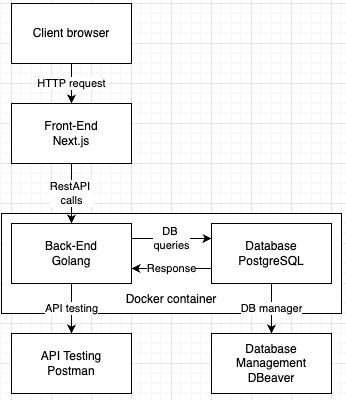
\includegraphics[]{src/images/image.png}
	\caption{Ажилтны Гүйцэтгэлийн Үнэлгээний Системийн Архитектурын Диаграм}
\end{figure}
\pagebreak